
\chapter{Автоматизация проектирования}

\section{Актуальность}

С увеличением количества интегрируемых IP-блоков в системах-на-кристалле (СнК), повышаются требования к узлам, отвечающим за их межсоединение.
Специфика разработки блоков межсоединения [{\color{red}более подробно в главе \ref{review}}].

Необходимость создания параметризированного по количеству как ведомых (slave), так и ведущих (master) портов межсоединения повлекла за собой работу по созданию средств для генерации RTL-описания.

\section{Научная новизна}

Генерация выходного RTL-описания IP-блоков по заданным параметрам реализована у многих вендоров. У большинства из них этот процесс заключается в создании RTL-описания в соответсвии со специфическим синтаксисом, расширяющим стандартный язык описания аппаратуры (например, Synopsys CoreBuilder или открытый проект CONfigurable NEtwork Creation Tool \cite{website:Connect}). Такой подход является зависимым от конкретного вендора и может быть применен только для IP-блоков той фирмы, которая занимается их разработкой совместно с разработкой средств для генерации.

Также вопросом реализации автоматизии процесса создания конфигурируемых IP-блоков занимались и независимые от вендоров команды (например, CoreTML framework). При этом решая проблему зависимости от поставщика IP-блоков, они не снимают все ограничения с процесса генерации. Так, в основе решения задачи сохраняется необходимость написание RTL-кода согласно со специфическим синтаксисом, что привязывает описание к конкретному программному средству генерации.

Подход, который предложен в данной работе, решает сформулированные проблемы:
\begin{enumerate}
  \item Зависимость от вендора.
  \item Зависимость от средств генерации.
\end{enumerate}

\section{Статьи и конференции}

На конференции в МФТИ был мой доклад на эту тему.

\section{Генерация RTL-описания}

\subsection{Описание подхода}

\subsection{Средства парсинга кода (lex, yacc)}

\subsection{Масштабирование кода}

Написано на языке go.

\subsection{GUI}

\begin{figure} [h]
  \center
  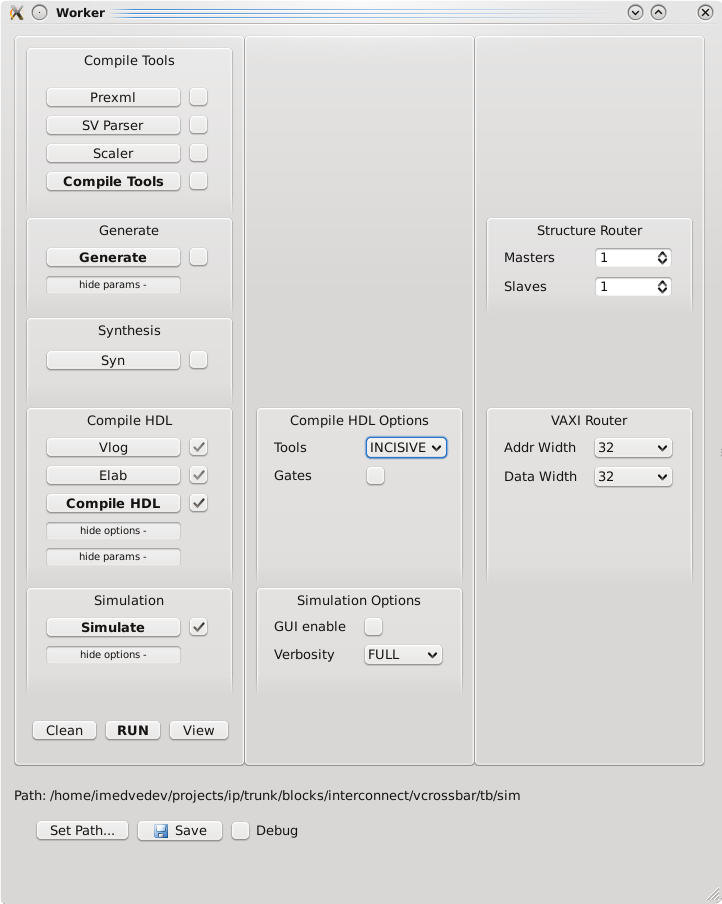
\includegraphics [scale=0.7] {pic01}
  \caption{GUI.}
  \label{img:pic01}
\end{figure}

\clearpage

